\chapter{Circuits séquentiels}
\section{Introduction}
Contrairement aux CLC (circuits logiques combinatoires), les sorties des les circuits logiques séquentiels ne dépendent pas que des entrées.
\subsection{Exemple}
Considérons le problème suivant: «on souhaite contrôler à l’aide d’un système logique la vanne de remplissage d’un réservoir. Le réservoir
dispose de deux capteurs 1 et 2 permettant de détecter le niveau maximal et le niveau minimal dans le réservoir.»\\
\begin{minipage}[t]{.5\textwidth}
Le système devrait assurer que
le niveau dans le réservoir ne soit
jamais au dessus de niveau
indiqué par le capteur 1 ($c_1$),
ni en dessous de niveau
indiqué par le capteur 2 ($c_2$).
\end{minipage}
\begin{minipage}{.5\textwidth}
	\begin{figure}[H]
		\centering
		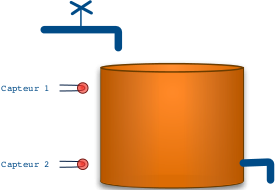
\includegraphics[width=.8\textwidth]{ch6/image1}
	\end{figure}
\end{minipage}
\ \\\\
Imaginons 2 situation:\\\\
\begin{minipage}{.5\textwidth}
	Réservoir plein en train de se vider:
	\begin{figure}[H]
		\centering
		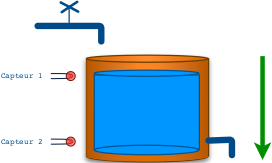
\includegraphics[width=.6\textwidth]{ch6/image2}
	\end{figure}
	\begin{table}[H]
		\centering
		$\begin{array}{c|c|c}
			$initial$ & $valeurs$ & $sortie$\\
			\hline
			\begin{array}{c}
				c_1=1\\
				c_2=1
			\end{array} & \begin{array}{c}
				c_1 = 0\\
				c_2=1
			\end{array} & 0
		\end{array}$
	\end{table}
\end{minipage}
\begin{minipage}{.5\textwidth}
	Réservoir vide en train de se remplir:
	\begin{figure}[H]
		\centering
		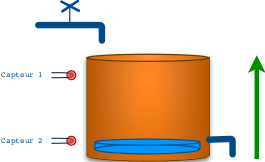
\includegraphics[width=.6\textwidth]{ch6/image3}
	\end{figure}
	\begin{table}[H]
		\centering
		$\begin{array}{c|c|c}
			$initial$ & $valeurs$ & $sortie$\\
			\hline
			\begin{array}{c}
				c_1=0\\
				c_2=0
			\end{array} & \begin{array}{c}
				c_1 = 0\\
				c_2=1
			\end{array} & 1
		\end{array}$
	\end{table}
\end{minipage}\ \\\\
Ainsi, pour une même combinaison d'entrées, nous avons 2 sorties!\\
Il nous faut mémoriser d'où est-ce que l'on vient $\Rightarrow$ notion d'état.
\subsubsection{Représentation avec les états}
\begin{figure}[H]
	\centering
	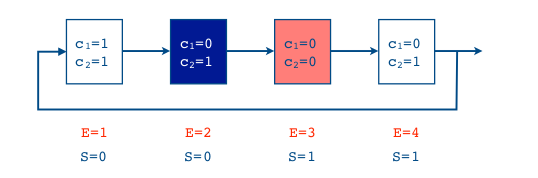
\includegraphics[width=.8\textwidth]{ch6/image4}
\end{figure}
Si les entrées sont:
\begin{itemize}
	\item $01$ ET l'état 2 $\Rightarrow$ ne rien faire.
	\item $01$ ET l'état 4 $\Rightarrow$ garder la pompe enclenchée.
\end{itemize}
Imaginons le système dans l'état 2 (état présent). Si $c_2=0$ alors le système va se trouver dans l'état 3 (état futur). On passe d'un état à l'autre (succession d'état).
\section{Systèmes séquentiels formellement}
Les sorties de ces systèmes dépendent aussi de l'état interne. Ils décident de leurs états futurs en fonction des entrées ET de leurs états présents.\\
La différence entre l'état futur et l'état présent (notion de \textit{rétroaction}) s'explique par la notion de délais (ajout de temps de propagation)
\begin{figure}[H]
	\centering
	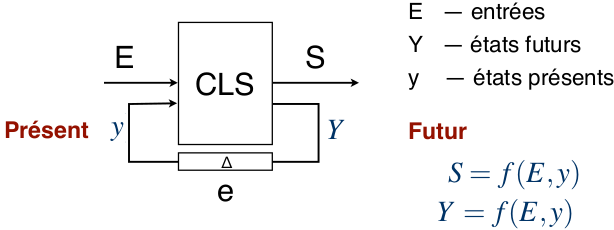
\includegraphics[width=.7\textwidth]{ch6/image5}
\end{figure}
\section{Représentation des systèmes séquentiels}
Il existe 3 modes de représentation:
\begin{itemize}
	\item Graphe d'état
	\item Table d'état (table de Huffman, matrice de transition)
	\item Équations logiques
\end{itemize}
La résolution de problème se fera donc: 
$$ \text{Cahier de charges verbal}\rightarrow\text{Table d'états}\rightarrow\text{Fonctions logiques}\rightarrow\text{Réalisation} $$
\subsection{Graphe d'état}
Dans ce mode de représentation on distingue:
\begin{itemize}
	\item Les états par des \textbf{cercles}
	\item Le passage d'un état stable à un autre par un \textbf{arc orienté} au-dessus duquel on note la(les) \textbf{condition(s)} sur les entrées impliquant la \textbf{transition}
\end{itemize}
\subsubsection{Exemple}
Voici un exemple d'un système à 4 états et 2 entrées
\begin{figure}[H]
	\centering
	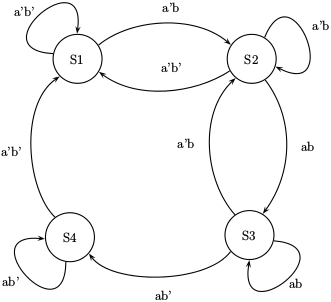
\includegraphics[width=.4\textwidth]{ch6/image6}
	\caption{Graphe d'état}
	\label{fig:graphetat}
\end{figure}
\subsection{Table de Huffman}
La table de Huffman indique l'évolution d'état du système (nb lignes = nb d'états). On distingue:
\begin{itemize}
	\item La première colonne indiquant les \textbf{états présents}
	\item Le reste des colonnes représentant toutes les possibilités des variables d'entrées
	\item Les états stables en \textbf{gras} ou entouré
	\item Les états de transition
\end{itemize}
\begin{figure}[H]
	\centering
	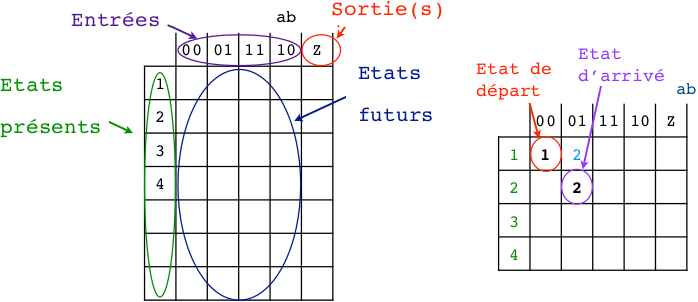
\includegraphics[width=.8\textwidth]{ch6/image7}
\end{figure}
\subsubsection{Graphe d'état à table d'état}
À partir du graphe de la \autoref{fig:graphetat}
on obtient
\begin{figure}[H]
	\centering
	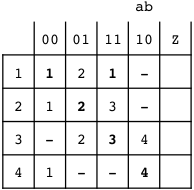
\includegraphics[width=.3\textwidth]{ch6/image8}
\end{figure}
remarquons que les transitions non-existantes sont marquées avec des \textit{don't care} (-)
\subsubsection{Lecture d'une table de Huffman}
Soit un système dans l'état 1, les entrées à $00$. Comme l'état l'état 1 à $00$ est stable, on y reste.\\
Imaginons que les entrées $ab$ changent de $00$ à $01$. Le système se comporte comme suivant:
\begin{figure}[H]
	\centering
	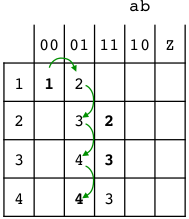
\includegraphics[width=.3\textwidth]{ch6/image9}
\end{figure}
On finit donc à l'état 4, stable pour les entrées $01$.
\subsubsection{Hypothèse sur les changements des entrées}
Voici les hypothèses:
\begin{enumerate}
	\item Le nombre de transitions entre 2 états stables n'est pas limité
	\item \textbf{On considère qu'entre 2 états stables (transitions) les entrées du système ne changent pas}
\end{enumerate}
La 2\up{ème} est très importante, si elle n'est pas respectée, le comportement du système devient imprévisible.\\
Dans la \autoref{fig:transit}, les entrées changent de $00\rightarrow 01\rightarrow 11$. La flèche verte représente la 1\up{ère} transition, la rouge la 2\up{ème} avant la fin de la première, la bleue après la fin de la première.
\begin{figure}[H]
	\centering
	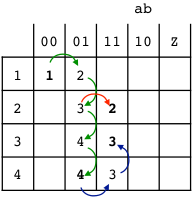
\includegraphics[width=.3\textwidth]{ch6/image10}
	\caption{Changement d'entrées lors des transitions}
	\label{fig:transit}
\end{figure}
On se retrouve donc dans des états différents pour une «même» transition
\paragraph{Remarque} Bien que le graphe d'état et la table de Huffman soient équivalents au niveau formel, on préférera la table car lors de son écriture, toutes les possibilités y sont représentées, alors qu'il est facile d'en oublier sur le graphe d'état.